\subsection{Processdir}
What you will quickly notice when tracing through the above diagram (Figure 3) the major functionality from this code comes from the processdir function. This function is where the -E -S and -T flags are processed. Therefore, this is where all of the SQL database accesses occur. This process is parallelized via a thread pool and is further optimized by a calculated rollupscore to ensure that we only descend into necessary sub-directories.

\subsection{querydb}
querydb is the macro used to execute sqlite commands


\begin{figure} [h]
\centering
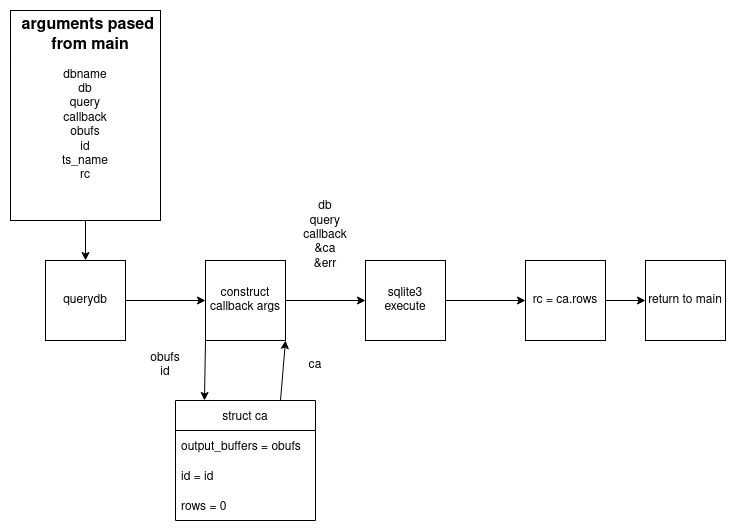
\includegraphics[width=0.8\textwidth]{images/querydb.png}
\caption{\label{fig:querydb}querydb workflow}
\end{figure}


\clearpage